\section{Planejamento das Atividades}

Para a realização desse trabalho, foram identificadas algumas atividades que deveriam seguir uma ordem para ser executadas, como mostra o diagrama a seguir:

\begin{figure}[h]
    \centering
    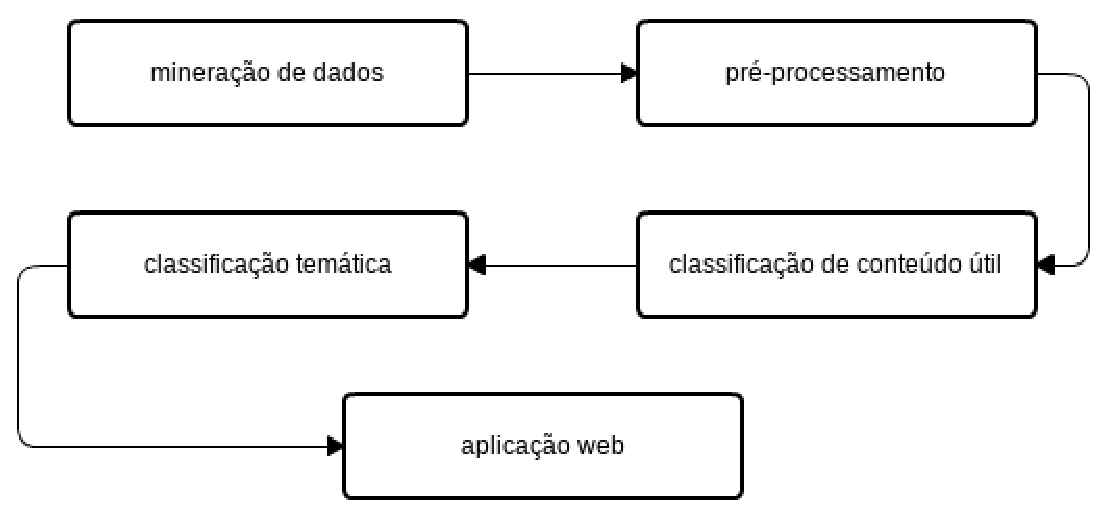
\includegraphics[scale=0.5]{figuras/planejamento.eps}
    \caption{Diagrama de planejamento}
\end{figure}

\subsection{Mineração de Dados}

A obtenção e persistência dos dados será realizada por uma biblioteca desenvolvida pelo autor, descrita na seção \ref{obtencao-dados}.

A obtenção dos dados consiste em realizar consultas ao \textit{webservice} da Câmara dos Deputados, fazendo um processamento inicial, afim de padronizar as informações e transformá-las em seus tipos correspondentes na linguagem \textit{python}. Os dados provenientes do \textit{webservice} estão em formato \textit{XML} e armazenam valores como \textit{strings}.

Nesta etapa transformamos todos os campos com valores de números inteiros e decimais, datas, horários e textos em, respectivamente, valores dos tipos \textit{int}, \textit{float}, \textit{datetime.date}, \textit{datetime.time} e \textit{str}.

\subsection{Pré-processamento}

Apesar do ``pré-processamento'' não depender tanto dos dados reais, a definição das \textit{stop words} deve ser feita levando em consideração o conteúdo que será analisado.

A etapa de pré-processamento consiste na análise dos textos obtidos na mineração de dados, afim de identificar as \textit{stop words} presentes em textos do contexto legislativo. Além disso, deve ser realizada o processo de \textit{stemização} para reduzir a dimensionalidade das \textit{bag-of-words} geradas.

Estudamos diferentes estratégias para a utilização de \(n\)-gramas, mas por enquanto decidiu-se, por uma questão de simplicidade, limitar-se apenas ao uso de unigramas.

\subsection{Classificação Conteúdo Útil}

Essa classificação tem como objetivo melhorar a qualidade da análise temática dos deputados. Uma parte considerável dos textos não possuem valor semântico significativo, pois tratam de questões protocolares e de trâmite legislativo. Citamos um exemplo: \textit{``É preciso haver quórum de 257 Srs. Deputados para aprovação da matéria, quórum mínimo. A votação é normal. Então, acho que, quando houver uns 300 ou 320 votos, encerraremos.''}. Portanto, a classificação entre conteúdo útil/não-útil consiste em separar os parágrafos que realmente possuem valor para a análise posterior dos que não devem ser usados nestas análises.

\subsection{Classificação Temática}

Após determinar quais parágrafos serão análisados, os mesmos devem ser classificados de acordo com alguns temas. Selecionamos inicialmente: Agropecuária, Saúde, Esporte, Educação, Ciência e Tecnologia, Economia, Política, Meio Ambiente, Direitos Humanos e Segurança. Para a realização dessa tarefa, foi necessário construir um texto inicial para cada um dos temas listados, afim de fornecer um parâmetro inicial ao classificador. Os textos iniciais de cada tema têm como base textos previamente classificados em portais de notícias brasileiros e consistem em apenas uma listagem de palavras comuns relacionadas a estes temas.

\subsection{Aplicação \textit{Web}}

Os dados obtidos da classificação temática serão utilizados para alimentar um sistema \textit{web} para a exibição dos
mesmos. As principais funcionalidades planejadas são: visualizar os temas mais abordados por deputados, organizados por região, partido e bancada, visualizar todos os temas de uma determinada categoria, bem como o quanto cada tema é discutido e visualizar todos os temas abordados por um determinado deputado, mostrando separadamente os temas abordados em seus discursos e nas suas proposições.

Esta parte do projeto está em fase inicial e não iniciou o desenvolvimento propriamente dito. As funcionalidades planejadas e protótipos iniciais estão disponíveis no apêndice \ref{prototipos-apendice}.
